% sample.tex
\documentclass{beamer}

\usetheme{boxes}

\usecolortheme[RGB={34,170,34}]{structure} 
\usepackage{amsmath}
\usepackage{amssymb}
\usepackage{graphics}
\usepackage{multicol}
\usepackage{color}
\usepackage[absolute,overlay]{textpos}
\usepackage{fancybox}

\usepackage{framed,color}
\definecolor{shadecolor}{rgb}{255,127,0}
\setbeamertemplate{itemize item}[circle]

\definecolor{verde}{RGB}{34,170,34}


\setbeamercolor{uppercolgreen}{fg=white,bg=verde!90}
\setbeamercolor{lowercolgreen}{fg=black,bg=verde!20}


%%%%%%%%%%%%%%%%%%%%%%%%%%%%%%%%%%%


\title[Shell Lesson]{Programming with Python}

\subtitle[]{EOAS Software Carpentry Workshop }
\date[Sep 2015]{September 24nd, 2015}


%------------------ the document starts here -------------------------%

\begin{document}
\bibliographystyle{plainnat}
\bibliography{bib/biblio}


%------------------ the titlepage frame-------- -------------------------%

 
\begin{frame}[plain]
  
\titlepage


\end{frame}


%---------------- the presentation begins here --------------------%

%-------------------------- Cool xkcd cartoon ------------------------------------------%

\begin{frame}

\begin{figure}[htbp]
   \centering
  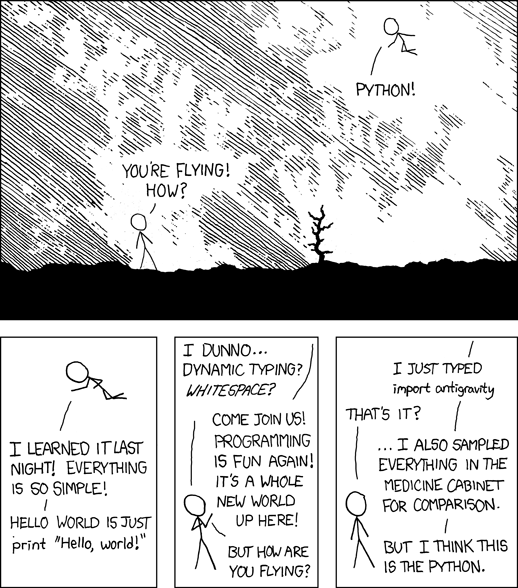
\includegraphics[width=0.6\textwidth]{figs_slides/python_xkcd.png} 
\end{figure}

\begin{textblock*}{7cm}(6.0cm,9.0cm)
		\centering
			\tiny{https://xkcd.com/353 }
\end{textblock*}



\end{frame}
%-------------------------- Intro ------------------------------------------%


\begin{frame}{Getting started}

\small{For our Python introduction we're going to pretend to be a researcher studying inflammation in patients who have been given a new treatment for arthritis.}
\vspace{0.5cm}

You need to download some files to follow this lesson:
\begin{enumerate}
 \item{Make a new folder in your Desktop called \texttt{python-novice-inflammation}.}
    \item{Download python-novice-inflammation-data.zip and move the file to this folder.}
    \item{If it's not unzipped yet, double-click on it to unzip it. You should end up with a new folder called data.}
   \item{You can access this folder from the Unix shell with:}
\end{enumerate}
\texttt{\$ cd \&\& cd Desktop/python-novice-inflammation/data}




\end{frame}

%-------------------------- jupyter notebook ------------------------------------------%

\begin{frame}{Launching Ipython (Jupyter) Notebook}

\small{There are several ways that we can use Python.  We're going to start with
a tool called Python Notebook that runs in the browser.
In a shell window enter these commands:}

\vspace{0.5cm}

\begin{beamerboxesrounded}[upper=uppercolgreen,lower=lowercolgreen,shadow=false]{}
\texttt{\$ cd \\
\$ cd Desktop/python-novice-inflammation/data \\
\$ ipython notebook}
\end{beamerboxesrounded}
\vspace{0.5cm}

\small{The shell window is now running a local web server for you.  Don't close it. You will need to open another shell window to do other command line things. Your browser should open to an "Jupyter:  Notebook" page showing a list of directories.}
\end{frame}

%-------------------------- AXIS ------------------------------------------%

\begin{frame}{Analyzing patient data}

\begin{enumerate}
    \item{Explain what a library is, and what libraries are used for.}
    \item{Load a Python library and use the things it contains.}
    \item{Read tabular data from a file into a program.}
    \item{Assign values to variables.}
    \item{Select individual values and subsections from data.}
   \end{enumerate}

\begin{multicols}{2}
\begin{itemize}
\item import numpy
\item numpy.loadtxt(fname=  delimiter=)
\item weight\_kg = 55
\item print('weight in kg:', weight\_kg)
\item weight\_lb = 2.2 * weight\_kg
\item type(data)
\item data.shape
\item data[0,0], data[0:1,0:1]
\item data[0:10:2,1]
\item data[:3,36:]
\end{itemize}
\end{multicols}
\end{frame}

%-------------------- intro 2 ---------------------------
\begin{frame}
\frametitle{Analyzing Patient Data cont'd}
\begin{enumerate}
\setcounter{enumi}{5}
\item    Perform operations on arrays of data.
\item    Display simple graphs.
\end{enumerate}
\begin{multicols}{2}
\begin{itemize}
\item data.mean()
\item data.std()
\item data.mean(axis=0)
\item \%matplotlib inline
\item from matplotlib import pyplot
\item pyplot.imshow(data)
\item pyplot.show()
\item pyplot.plot(ave\_inflammation)
\item import matplotlib import pyplot as plt
\item plt.subplot(1,3,1)
\item plt.ylabel('average')
\item plt.show()
\end{itemize}
\end{multicols}
\end{frame}




%-------------------------- AXIS ------------------------------------------%

\begin{frame}{Operations across an axis}

\begin{figure}[htbp]
   \centering
  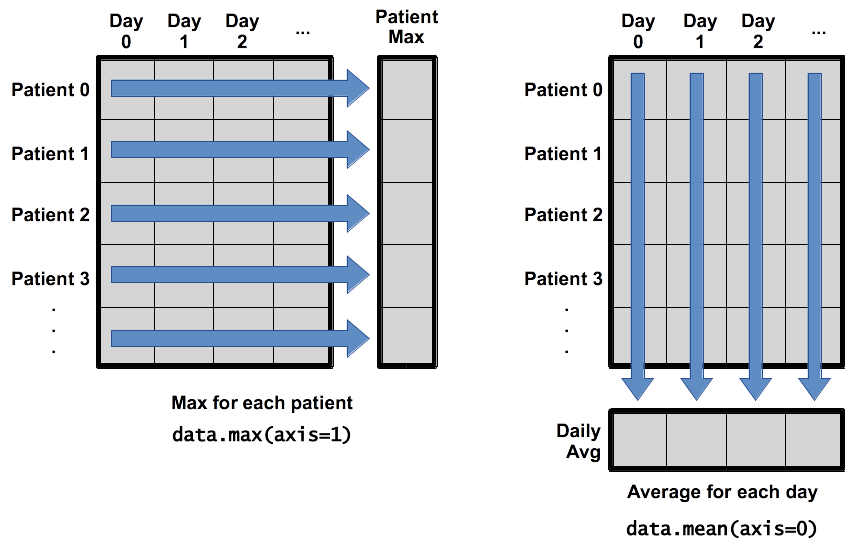
\includegraphics[width=0.7\textwidth]{figs_slides/python-operations-across-axes.png} 
\end{figure}

\end{frame}


%%-------------------------- Challenge 01 ------------------------------------------%

\begin{frame}{Exercise}
Create a single plot showing 1) the mean for each day and 2) the mean + 1 standard deviation for each day and 3) the mean - 1 standard deviation for each day.

\end{frame}

%% ---------------------------------- LOOPS ----------------------------------------%
\begin{frame}{Repeating actions with loops}

\begin{enumerate}
    \item{Explain what a for loop does.}
    \item Correctly write for loops to repeat simple calculations.
    \item{Trace changes to a loop variable as the loop runs.}
    \item{Trace changes to other variables as they are updated by a for loop.}
   \end{enumerate}

\begin{multicols}{2}
\begin{itemize}
\item for char in word:
\item len('aeiou')
\end{itemize}
\end{multicols}
\end{frame}
%-------------------------- Challenge 02 - loops ------------------------------------------%

\begin{frame}{ }

Python has a built-in function called range that creates a list of numbers: range(3) produces [0, 1, 2], range(2, 5) produces [2, 3, 4], and range(2, 10, 3) produces [2, 5, 8]. Using range, write a loop that prints the first three natural numbers:

\vspace{0.5cm}

\begin{beamerboxesrounded}[upper=uppercolgreen,lower=lowercolgreen,shadow=false]{}
\texttt{1\\
2\\
3}
\end{beamerboxesrounded}

\end{frame}

%-------------------------- Challenge 05 - loops - My Sol------------------------------------------%

\begin{frame}{ }

Python has a built-in function called range that creates a list of numbers: range(3) produces [0, 1, 2], range(2, 5) produces [2, 3, 4], and range(2, 10, 3) produces [2, 5, 8]. Using range, write a loop that prints the first three natural numbers:

\vspace{0.5cm}

\alert{One solution:}

\texttt{for num in range(1,4,1):}

\texttt{      print(num)}
    

\end{frame}


%-------------------------- Challenge 06 - loops ------------------------------------------%

\begin{frame}{ }

Exponentiation is built into Python:

\vspace{0.5cm}

\begin{beamerboxesrounded}[upper=uppercolgreen,lower=lowercolgreen,shadow=false]{}

\texttt{print(5**3)\\
125}
\end{beamerboxesrounded}

\vspace{0.5cm}

Write a loop that calculates the same result using multiplication (without exponentiation).
\end{frame}

%%-------------------------- Challenge 06 - loops - My Solution ------------------------------------------%

\begin{frame}{ }

Exponentiation is built into Python:

\vspace{0.5cm}

\begin{beamerboxesrounded}[upper=uppercolgreen,lower=lowercolgreen,shadow=false]{}

\texttt{print(5**3)\\
125}
\end{beamerboxesrounded}

\vspace{0.5cm}

Write a loop that calculates the same result using multiplication (without exponentiation)

\alert{One possible answer:}

\texttt{ans=1}\\
\texttt{for ii in range(1,4,1):}\\
\texttt{      ans=ans*5}\\
\texttt{print(ans)}

\end{frame}

%-------------------------- the document ends here ----------------------------------%

\end{document}
